% !TeX spellcheck = en_US
\documentclass[letterpaper,12pt,twoside]{report}
\usepackage{fancyhdr}
\usepackage{fullpage}
\usepackage{tikz}
\usepackage{amsmath}

\begin{document}
	\pagestyle{fancy}
	\fancyhf{}
	\fancyhead[L]{Day 5}
	\fancyhead[R]{\textit{The Calendar Project}}
	\fancyfoot[L]{Citations Involved: 2, 3}
	
	% Problem
	\paragraph{Problem}
	\begin{quote}
	\textsf{Consider the parabola with equation $y = x^2$ and the rectangle with vertices $(1,0)$, $(1,1)$, $(-1,1)$, and $(-1, 0)$. Find the area of the parabolic segment (shaded) and compare its area with that of the rectangle.}
	\end{quote}
	
	% Graphics
	\begin{minipage}{.45\linewidth}
	\begin{center}
		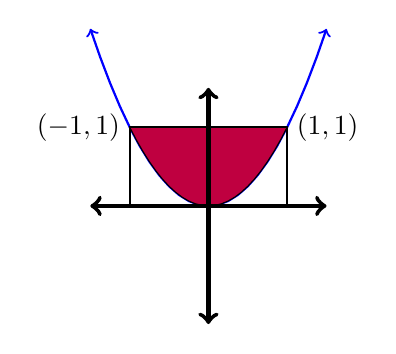
\begin{tikzpicture}
		
		\draw [<->][blue, thick, domain=-1.5:1.5] plot (\x, {\x*\x});
		\draw [thick] (-1,0) -- (-1, 1) -- (1, 1) -- (1, 0);
		\draw[fill=purple,domain=-1:1] (-1,1) -- plot ({\x},{\x*\x}) -- (1,1) -- cycle;
		
		\draw [<->][ultra thick] (-1.5,0) -- (1.5,0);
		\draw [<->][ultra thick] (0,1.5) -- (0,-1.5);
		
		\node[left] at (-1,1) {$(-1,1)$};
		\node[right] at (1,1) {$(1,1)$};
		\end{tikzpicture}
	\end{center}
\end{minipage}
\begin{minipage}{.45\linewidth}
	\begin{center}
		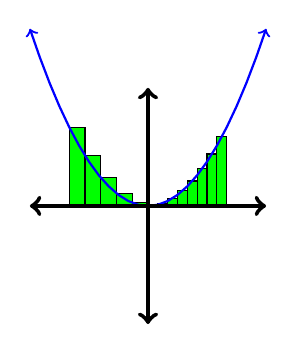
\begin{tikzpicture}
			\draw[fill=green] (-1,1) -- (-0.8,1) -- (-0.8,0) -- (-1,0) -- cycle;
			\draw[fill=green] (-0.8,0.64) -- (-0.6,0.64) -- (-0.6,0) -- (-0.8,0) -- cycle;
			\draw[fill=green] (-0.6,0.36) -- (-0.4,0.36) -- (-0.4,0) -- (-0.6,0) -- cycle;
			\draw[fill=green] (-0.4,0.16) -- (-0.2,0.16) -- (-0.2,0) -- (-0.4,0) -- cycle;
			\draw[fill=green] (-0.2,0.04) -- (0,0.04) -- (0,0) -- (-0.2,0) -- cycle;
			\draw[fill=green] (0,0.00390625) -- (0.125,0.00390625) -- (0.125,0) -- (0,0) -- cycle;
			\draw[fill=green] (0.125,0.03515625) -- (0.25,0.03515625) -- (0.25,0) -- (0.125,0) -- cycle;
			\draw[fill=green] (0.25,0.09765625) -- (0.375,0.09765625) -- (0.375,0) -- (0.25,0) -- cycle;
			\draw[fill=green] (0.375,0.19140625) -- (0.5,0.19140625) -- (0.5,0) -- (0.375,0) -- cycle;
			\draw[fill=green] (0.5,0.31640625) -- (0.625,0.31640625) -- (0.625,0) -- (0.5,0) -- cycle;
			\draw[fill=green] (0.625,0.47265625) -- (0.75,0.47265625) -- (0.75,0) -- (0.625,0) -- cycle;
			\draw[fill=green] (0.75,0.66015625) -- (0.875,0.66015625) -- (0.875,0) -- (0.75,0) -- cycle;
			\draw[fill=green] (0.875,0.87890625) -- (1,0.87890625) -- (1,0) -- (0.875,0) -- cycle;
			\draw[<->][blue,thick,domain=-1.5:1.5] plot (\x,{\x*\x});
			
			\draw [<->][ultra thick] (-1.5,0) -- (1.5,0);
			\draw [<->][ultra thick] (0,1.5) -- (0,-1.5);
		\end{tikzpicture}
	\end{center}
\end{minipage}

	\paragraph{Summation Notation (Sigma)}
	\begin{quotation}
		The summation symbol, or uppercase Sigma in the Greek alphabet, represents the collective sum of the expression immediately following it for all values of the counter variable from the specified starting value to the ending value. It is more formally defined as follows: $$\sum^n_{i=j}f(i)=f(j)+f(j+1)+f(j+2)+\dots+f(n-1)+f(n)$$
		
		
	\end{quotation}
	\paragraph{The Limit Notation}
	\begin{quotation}
		In modern mathematics (especially Calculus), there are certain expressions that produces an unwanted value when certain variables reach certain values. A basic example of this is division by zero, which evaluates to undefined. The limit notation is used to describe what the value of the expression \textbf{approaches} as a certain variable approaches a certain value. In this example, the following expression would be used with the notation: $$\lim_{n\to 0} \frac{1}{n}(=\infty)$$
		
		\textit{As $n$ approaches 0, $\frac{1}{n}$ approaches $\infty$}. Note that this notation can also be applied to normal expressions; an example of this is shown below: $$\lim_{n \to 10} 20n=20\cdot10=200$$
		
		The limit notation is an important concept in Calculus as it captures the notion of \textit{minimizing a value}. It will be revisited frequently.
	\end{quotation}
	
	\begin{center}
		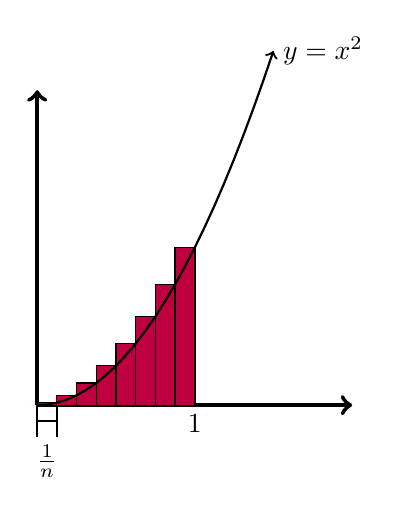
\begin{tikzpicture}[scale=2]
			\draw[->,ultra thick] (0,0) -- (0,2);
			\draw[->,ultra thick] (0,0) -- (2,0);
			
			\draw[thick] (1,1) -- (1,0);
			\draw[fill=purple] (0,{0.125*0.125}) -- (0.125,{0.125*0.125}) -- (0.125,0) -- (0,0) -- cycle;
			\draw[fill=purple] (0.125,{0.25*0.25}) -- (0.25,{0.25*0.25}) -- (0.25,0) -- (0.125,0) -- cycle;
			\draw[fill=purple] (0.25,{0.375*0.375}) -- (0.375,{0.375*0.375}) -- (0.375,0) -- (0.25,0) -- cycle;
			\draw[fill=purple] (0.375,0.25) -- (0.5,0.25) -- (0.5,0) -- (0.375,0) -- cycle;
			\draw[fill=purple] (0.5,{0.625*0.625}) -- (0.625,{0.625*0.625}) -- (0.625,0) -- (0.5,0) -- cycle;
			\draw[fill=purple] (0.625,{0.75*0.75}) -- (0.75,{0.75*0.75}) -- (0.75,0) -- (0.625,0) -- cycle;
			\draw[fill=purple] (0.75,{0.875*0.875}) -- (0.875,{0.875*0.875}) -- (0.875,0) -- (0.75,0) -- cycle;
			\draw[fill=purple] (0.875,1) -- (1,1) -- (1,0) -- (0.875,0) -- cycle;
			\draw[->,thick,domain=0:1.5] plot ({\x},{\x*\x});
			\node[below] at (1,0) {$1$};
			
			\draw[thick] (0,0) -- (0,-0.2);
			\draw[thick] (0.125,0) -- (0.125,-0.2);
			\draw[thick] (0,-0.1) -- (0.125,-0.1);
			\node[below] at (0.0625,-0.19) {$\frac{1}{n}$};
			\node[right] at (1.5,2.25) {$y=x^2$};
		\end{tikzpicture}
	\end{center}
	\paragraph{Riemann Sums}
	\begin{quotation}
		Given a graph of $y=f(x)$, The area under a curve can be approximated using a method named Riemann Sums, in which the area is horizontally split into an arbitrary number of rectangles. See the figure near the problem definition on the right for an example. To prevent further complication, the optimal approach with this method is where each rectangle has equal width; this approach will be used below.
		
		The accuracy of approximation using Riemann Sums increases when more rectangles are used; when the number of rectangles approaches $\infty$, the deduced area approaches the exact answer.
		
		In this problem, the graph is given to be $y=x^2$. From the Area Addition Postulate, it can be deduced that the shaded area is equal to the area of the bounding rectangle (with the given vertices) subtracted from the exact area bounded by $y=x^2$, the $x$-axis, $x=-1$, and $x=1$. For simplicity, the area of the region bounded by $y=x^2$, the $x$-axis, the $y$-axis, and $x=1$ is determined below; the deduced area is later used to find the answer to this problem.
		
		Let the number of rectangles be $n$, and let $x_i$ represent the $x$ component of the vertical line that contains the \textbf{right} side of the $i^\text{th}$ rectangle, where $1\leq i\leq n$. Let the height of the $i^\text{th}$ rectangle be determined by $f(x_i)$; in this problem, this is equal to $x_i^2$. Let the width of the rectangles be $w$; with $n$ rectangles, the width of the composite shape can be represented by $wn$; it is given that $wn=1-0=1 \Rightarrow w=\frac{1}{n}$. Given that the left boundary of the area being determined is the $y$-axis, the left side of the first rectangle is located on the $y$-axis. Since each rectangle has a width of $\frac{1}{n}$, the $x$ component of the vertical line containing the right side of the $i^\text{th}$ rectangle can be represented by $i\frac{1}{n} \Rightarrow \frac{i}{n}$; as such, $x_i=\frac{i}{n}$.
		
		To determine the expression for $x_i$, The area formula for a rectangle is its width multiplied by its height; as such, the area of the $i^\text{th}$ rectangle can be represented by $(\frac{1}{n})(x_i^2)$. The sum of the area of the rectangles can therefore be represented by $(\frac{1}{n})(x_1^2)+(\frac{1}{n})(x_2^2)+(\frac{1}{n})(x_3^2)+\dots+(\frac{1}{n})(x_n^2)$; by the distributive property, this can be simplified to $(\frac{1}{n})(x_1^2+x_2^2+x_3^2+\dots+x_n^2)$, or $\frac{1}{n}\sum^n_{i=1} x_i^2$. Additionally, to determine the \textbf{exact} area of the region, the number of rectangles must be maximized. As such, using $\frac{i}{n}$ as a substitute for $x_i$, the area of this region can be expressed and transformed as follows:
		\begin{align*}
		\lim_{n\to\infty}\frac{1}{n}\sum^n_{i=1}(\frac{i}{n})^2 &= \lim_{n\to\infty}\frac{1}{n}\sum^n_{i=1}\frac{i^2}{n^2} \\
		&= \lim_{n\to\infty}\frac{1}{n}\frac{\sum^n_{i=1}i^2}{n^2} \\
		&= \lim_{n\to\infty}\frac{\sum^n_{i=1}i^2}{n^3}
		\end{align*} 
		
		One of Bernoulli's formulas, $\sum_{k=0}^{n}k^2=\frac{n(n+1)(2n+1)}{6}$, can be used. Since the first term of the expanded expression of the summation, $0^2$, is 0, this formula also equals to $\sum_{k=1}^{n}$ by the Addition Property of Zero. After substitution, the final form above is transformed as follows:
		
		\begin{align*}
		\lim_{n\to\infty}\frac{\sum^n_{i=1}i^2}{n^3}
		&= \lim_{n\to\infty}\frac{\frac{n(n+1)(2n+1)}{6}}{n^3} \\
		&= \lim_{n\to\infty}\frac{n(n+1)(2n+1)}{6n^3} \\
		&= \lim_{n\to\infty}\frac{2n^3+3n^2+n}{6n^3} \\
		&= \lim_{n\to\infty}\frac{2n^2+3n+1}{6n^2} \\
		&= \lim_{n\to\infty}(\frac{2n^2}{6n^2}+\frac{3n}{6n^2}+\frac{1}{6n^2}) \\
		&= \lim_{n\to\infty}(\frac{1}{3}+\frac{1}{2n}+\frac{1}{6n^2})
		\end{align*}
		
		As $n$ approaches $\infty$, fractions whose denominators include $n$ as a multiplicative term approach $0$ in value. As such, the final expression above can be simplified to $(\frac{1}{3}+0+0)=\frac{1}{3}$. Since squares have the property that $(-x)^2=x^2$, the given parabola is symmetric across the $y$-axis. As such, reusing this strategy for the area bounded by $y=x^2$, the $y$-axis, the $x$-axis, and $x=-1$ yields the same result of $\frac{1}{3}$. By the Area Addition Postulate, the area under $y=x^2$ from $x=-1$ to $x=1$ is $\frac{1}{3}+\frac{1}{3}=\frac{2}{3}$.
		
		The rectangle is given to have vertices $(1,0)$, $(1,1)$, $(-1,1)$, and $(-1, 0)$. Its length is the distance between $(-1,0)$ and $(1,0)$, which is $\sqrt{(1-(-1))^2+(0-0)^2}=\sqrt{2^2}=2$. Its width is the distance between $(-1,0)$ and $(-1,1)$, which is $\sqrt{(-1-(-1))^2+(0-1)^2}=\sqrt{0+1}=1$. The formula for the area of a rectangle is its length multiplied by its width, or $2\cdot 1=2 \text{  units}^2$. By the Area Addition Postulate, the sum of the area of the given shaded parabolic segment and the area under the parabola that is previously determined equals the area of the rectangle: $[\text{given parabolic segment}]+\frac{2}{3}=2 \Rightarrow [\text{given parabolic segment}]=2-\frac{2}{3}=\frac{4}{3}$. The area of the given parabolic segment compared to the the area of the rectangle is therefore $\frac{\frac{4}{3}}{2}=\boxed{\frac{2}{3}}$.
	\end{quotation}

\end{document}